% ---- ETD Document Class and Useful Packages ---- %
\documentclass{ucetd}
\usepackage{subfigure,epsfig,amsfonts}
\usepackage{natbib}
\usepackage{amsmath}
\usepackage{amssymb}
\usepackage{amsthm}
\usepackage[toc,page]{appendix}

\usepackage{url}


%% Use these commands to set biographic information for the title page:
\title{Stochastic computation in recurrent networks of spiking neurons}
\author{Clayton W. Seitz}
\department{Graduate Program in Biophysics}
\division{Physical and Biological Sciences}
\degree{Master of Science}
\date{Winter 2021}

%% Use these commands to set a dedication and epigraph text

\epigraph{Epigraph}

\begin{document}
%% Basic setup commands
% If you don't want a title page comment out the next line and uncomment the line after it:
\maketitle
%\omittitle

% These lines can be commented out to disable the copyright/dedication/epigraph pages
\makecopyright
%\makededication
\makeepigraph


%% Make the various tables of contents
\tableofcontents
%\listoffigures
%\listoftables

\acknowledgments
% Enter Acknowledgements here

\abstract

The primate cerebral cortex is a complex system estimated to harbor more than 25 billion neurons communicating via action potentials or `spikes' and is responsible for many higher-order brain functions including memory and learning. Recent years have hosted many efforts to understand how such complex phenomena emerge from the communication of individual cells. Many studies have provided evidence that long term plasticity (LTP) in synapses permits a long-lasting alteration of network dynamics and, in turn, forms the basis of long-term memory and learning. However, understanding memory formation and learning in the brain is made difficult by the variability in the response of cortical neurons to stimuli. Therefore, capturing the apparent stochastic features of neural activity in computer based models, such as recurrent spiking neural networks (RSNNs), while explaining their manipulation of information mathematically has become the gold standard for computational neuroscience. Models of neural networks derived from statistical mechanics, such as those which assert that the membrane potential of a cortical neuron obeys a form of Langevin dynamics, can potentially account for stochastic network activity. Such models also provide the intriguing interpretation that neural activity represents sampling from a probability distribution - a technique central to statistical inference.  Here, we apply a similiar mathematical treatment to the study of an RSNN by modeling the membrane potential statistics of an integrate and fire neuron using Fokker-Planck equations. With this statistical framework in hand, we can recast a network of neurons as a stochastic process in higher dimensions and explore the relationships between synaptic connectivity and its plasticity to the correlation structure of neural spike trains. This approach is also amenable to information theoretic analysis and is a step toward a mathematical relationship between neuroplasticity mechanisms and the emergent computational capabilities of cortical microcircuits.



\mainmatter

\chapter{Models of action potential generation}

The dominating information processing unit in neocortex is the spiking neuron - a neural cell which exhibits transient depolarization of the cell membrane called action potentials or\emph{spikes}. The potential is regulated by a diverse set of highly specific ion channels embedded in the plasma membrane which open and close based on environmental factors such as the membrane potential itself or changes in the concentration of neurotransmitters. This dependence of the so-called \emph{open probability} of ion channels results in changes of the membrane conductance for the ions they transport and is the origin of the non-linear properties of  cells in the nervous system. Several mathematical models have been proposed to explain this process in various levels of detail, generally depending on their application. Some consider the biophysical details of action potential generation by considering specific types of ion channels and their dynamics while others neglect such details for the sake of mathematical simplicity. At the same time, models are often classified as conductance-based or current-based, depending on whether they model the membrane conductance explicitly or summarize membrane depolarization as a sum of membrane currents. The famous Hodgkin-Huxley (HH) model published in 1952 was originally used to fit experimental voltage traces measured in the squid giant axon and is arguably the most biophysically accurate of model of membrane depolarization. The membrane potential of an HH neuron evolves according to a a set of ordinary differential equations that include a term for each of the ion channels thought to be critical for the generation of an action potential. In the following paragraphs, we will briefly introduce the Hodgkin-Huxley model alongside an integrate and fire (IF) model to provide context for the following chapters.

\section{Integrate-and-Fire Neuron Models}

The integrate and fire (IF) model of a cortical neuron has become a standard tool for exploring neuronal dynamics. It's relative simplicity makes it an appealing choice for large scale simulations where the precise details of synaptic transmission can be neglected and a neuron can be described with only a few state variables. A large body of research has shown that precise timing of action potentials has an important role in neural information processing - a feature central to the IF model (Rieke, 1997). However, it is important to note that the IF model remains a coarse approximation to the diverse set of neurons observed thus far in cortex. Biophysical models such as the Hodgkin-Huxley model are known to describe action potential generation more precisely than IF models, but have the significant drawback that they are computationally expensive. Even the minimalist IF model presents substantial barriers to theoretical analysis (Brunel 2000). On the other hand, IF models have been shown to capture a diverse set of dynamical states observed in cortex (Citation). 

Noisy variants of IF models have been introduced to summarize the enormous number of degrees of freedom due to millions of ion channels and thousands of presynaptic signals impinging on the neuron (Tuckwell 1989, Plesser 2000). Such models describe the inputs to a neuron by decomposing the total synaptic input into a deterministic part $I(t)$ and a stochastic part $\xi(t)$, which is taken to be a gaussian white noise (GWN). 

\begin{align}
\tau\dot{V_{j}} = -V_{j} + \mu_{j}(t) + \xi_{j}(t)
\end{align}


with $\langle\xi(t)\xi(t')\rangle = \sigma^{2}\delta(t-t')$. The afferent currents $\mu(t)$ and $\xi(t)$ are interpreted as post-synaptic potentials (PSPs) and thus have dimensions of voltage. Eq. (1.1) has the form of a well-known stochastic differential equation (SDE) called the Langevin equation. When the voltage $V$ crosses a firing threshold $\Theta$, we say the neuron has fired an action potential and the voltage is reset to the resting value $V_{R}$. Therefore, we define an additional state variable $z(t) = H(V-v_{th})$ where $H$ denotes the Heaviside step function.


Stochasticity in IF neurons can be obtained through several mechanisms, such as a noisy reset potential, noisy firing threshold, or intrinsic noise originating in the stochastic features of membrane channels (Plesser and Gerstner 2000, Neftci 2014) or the exocytosis of synaptic vesicles. At the same time, stochastic spike arrival may contribute to fast fluctuations in the membrane potential that cannot be described by a deterministic component $I(t)$. Contrary to intuition, many have suggested that this randomness could contribute positively to the computational paradigm employed in cortical circuits. This phenomenon, referred to as \emph{stochastic resonance} is a property of a dynamical system subject to both periodic forcing and random perturbation may show a resonance only when both the periodic forcing and random perturbation are present (Benzi, 1981). In the context of IF models, the deterministic current $I(t)$ (the summation of post-synaptic potentials) may be subthreshold and $\xi(t)$ is required to push the membrane potential over threshold. Neurons in this regime have a large coefficient of variation just as cortical neurons (Konig, Engel, Singer 1996). More recently, additional evidence has been found that an optimal noise level coincides with the critical regime (Rodriguez 2017) a parameterization of the network that optimizes information transmission (Cramer 2020).

\section{The Ornstein-Uhlenbeck Process}

Langevin equations in the form of (1.1) have been studied extensively and their statistical features have been defined rigorously. In this form, they resemble the Ornstein-Uhlenbeck (OU) process, which is often used in statistical physics to describe a diffusing particle undergoing Brownian motion (Wiener process) with friction. In Brownian motion, the displacement of a variable $x$ in a time $dt$ is normally distributed with variance proportional to $\Delta t$ i.e. $V(t+dt) - V(t) \sim N(0, \sigma^{2}dt)$ or equivalently $dV \sim \sigma\sqrt{dt}\eta(t)$. The Ornstein-Uhlenbeck process is commonly written as a Langevin equation with a noise term similar to Brownian motion but with an added frictional term $-V(t)$ and a non-stationary white-noise $\mu(t) + \sigma\sqrt{dt}\eta(t)$ giving


\begin{equation}
\tau\dot{V_{j}}(t) = -V_{j}(t) + \mu_{j}(t) + \sigma_{j}\sqrt{dt}\eta(t)
\end{equation}

with $\eta(t) \sim \mathcal{N}(0,1)$. Note this equation is identical to (1.1) with $\xi_{j}(t) = \sigma_{j}\sqrt{dt}\eta(t)$. The last two terms in (1.2) are summarized by the total current arriving at the soma of a neuron $I_{j}(t) = \mu_{j}(t) + \sigma_{j}\sqrt{dt}\eta(t)$. Since (1.1) is stochastic, its solution is a probability distribution over the stochastic variable as a function of time $P(V,t)$. This distribution can be found by using the Kramers-Moyal Expansion (KME) which is derived in Appendix A. We state the result of that derivation here for brevity

\begin{align}
\tau\dot{P}(V,t) &= \frac{\partial}{\partial V}[\left(V(t)-\mu(t)\right) P(V,t)] + \frac{\sigma^{2}}{2}\frac{\partial^{2}}{\partial V^{2}}[P(V,t)]
\end{align}

An important difference in the IF model in (1.1) and the OU process is that the voltage variable $V$ in the IF model is bounded below by $V_{R}$ and above by the threshold $\theta$ while the OU process is unbounded, in general. The transition density $T(V',t'|V,t)$ has a known analytical form:

\begin{align*}
T(V',t+\Delta t|V,t) = \sqrt{\frac{1}{\tau\pi\sigma^{2}(1-\exp\left(-2\Delta t/\tau)\right))}}\exp\left(-\frac{1}{\tau\sigma^{2}}\frac{(V'-V_{R}\exp(-\Delta t/\tau))^{2}}{1-\exp\left(-2\Delta t/\tau\right)}\right)
\end{align*} 

This is equivalent to the distribution $P(V,t)$ as can be seen by plugging $T$ into (2.1) and setting the initial condition $P(V,t) = \delta(V-V_{R})$.

\begin{figure}
\centering
\subfigure[]{\label{fig:a}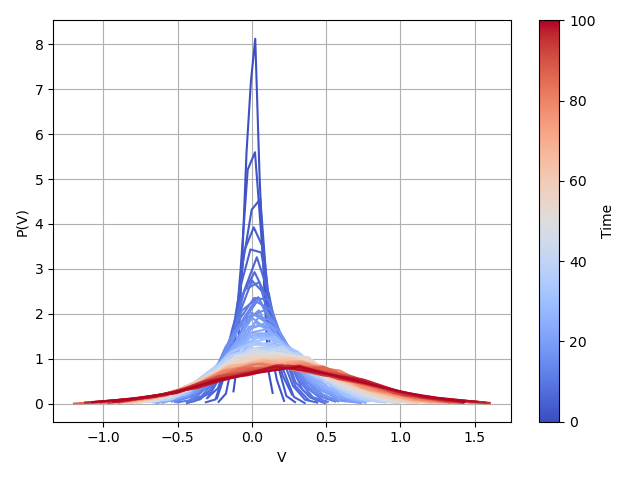
\includegraphics[width=80mm]{fig_1-A}}
\subfigure[]{\label{fig:b}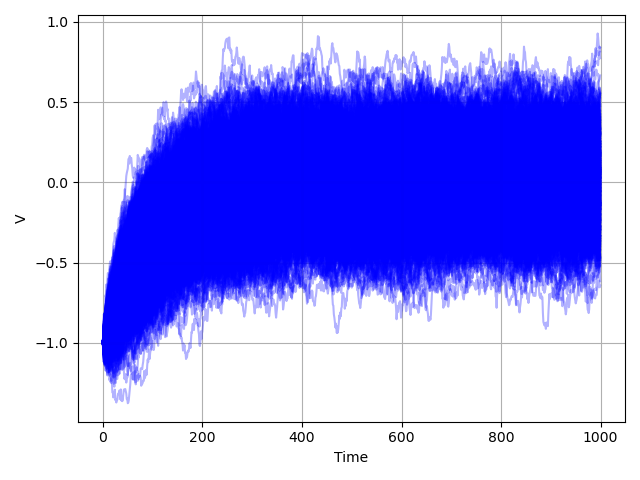
\includegraphics[width=80mm]{fig_1-B}}
\caption{Monte Carlo simulation of a Langevin equation for a gaussian white noise process with $\sigma = 1$, $\Delta t=0.002$, $\alpha=10$, and $V(0)=-1$. (a) Distribution of $V$ for $N=10,000$ units as a function of time (dashed is the theoretical prediction, solid is the simulation result). See stationary distribution in cyan (b) Time course for $N=10,000$ units}
\end{figure}

\section{Monte Carlo Simulations}

\chapter{Self-organization of complex systems}

Complex systems are ubiquitous in nature yet our scientific efforts have thus far only begun to gain traction on their governing principles. Many of the most intriguing complex systems in nature exihibit behaviors that simply cannot be explained by any of the components in isolation but rather arise from their complex interactions, bringing emergent phenomena into the focus of modern science. Such systems may be of physical, economic, or biological in nature, but all are thought to exihibit emergent properties under the appropriate conditions, suggesting broad relevance for the study of complex systems. 

To put complexity into perspective, consider the states of an interacting system of $N$ binary variables denoted $\{z_{i}\}_{i=1}^{N}$ which might be physically realized as an ensemble of spins in a ferromagnet. Even for extremely small cases such as $N=100$ the system can take on $2^{100} = 1.26\times 10^{30}$ different configurations and by $N=300$ the number of configurations exceed our best estimates for the number of atoms in the known universe. These unimaginabily large numbers simultaneously suggest that we cannot even hope to estimate a probability distribution over the phase space of the system, even with the most cutting edge experimental apparatus. The human cerebral cortex parallels this complexity, but maintains an order evident in the stability of our sensory percepts, in spite of its construction from over 16 billion noisy nerve cells. 

Neurons in cortex connect when afferent nerve fibers of a presynaptic cell meet a small patch of the dendritic tree or soma of a post-synaptic, forming the synapse. The complexity of neural networks arises from the complexity of these communication channels. It is a great challenge to understand how the complex connectivity patterns in cortex give rise to stable functions including the formation and retrieval of memories. In his famous neurophysiological postulate, Donald Hebb first proposed a cellular mechanism for the self-organization of networks of neurons [1]. Hebb suggested that repeated stimulation of specific receptors of sensory signals would lead slowly to the formation of a \emph{cell assembly} and these structural changes would constitute a representation or imprint of an internally or externally generated sensation e.g., an image or idea. This process, referred to as Hebbian learning, is argued to be driven by the temporal order of action potentials where the synaptic efficacy of the connection between neurons increases when a presynaptic neuron fires an action potential before a postsynaptic neuron.

\section{Synaptic plasticity as the basis for memory and learning}

Synaptic plasticity refers to the activity-dependent modification of the strength or efficacy of synaptic transmission at preexisting synapses, and has been proposed to play a central role in the incorporation of transient experiences into persistent memory traces. The efficacy of an excitatory synapse can be either potentiated or depressed by a variety of mechanisms which occur over a wide range of time scales: from milliseconds to hours to days. Short-term synaptic plasticity (STP) is thought to play an important role in information processing in the brain. Its duration allows STP to modify the response of cortical circuits to stimuli and potentially provide a richer set of response properties without permanently altering the circuit architecture. One of several mechanisms thought to underly STP can be seen by the repeated stimulation of a presynaptic cell causing a transient accumulation of calcium in the presynaptic terminal (Mongillo et al. 2008). Calcium generally thought to elevate the probability of neurotransmitter release due to its proposed interaction with the biochemical machinery involved in synaptic vesicle excytosis. Other short term changes in synaptic efficacy can occur such as the facilitation or depression based upon the temporal characteristics of the stimulus. In paired-pulse experiments, a pair of stimuli is delivered a sub-20ms interval shows depression of the efficacy of the second stimulus (Zucker and Regehr, 2002). This phenomenon is hypothesized to arise from inactivation of voltage-dependent sodium and/or calcium channels or depletion of the release ready pool of synaptic vesicles at the presynaptic terminal [1]. Synaptic efficacy can be lowered by the release of biochemical modulators which can interact with the synaptic machinery to inhibit the release of neurotransmitter into the synaptic cleft. In addition, receptors at the presynaptic terminal which play a role in the secretion of neurotransmitter are sensitive to the presence of presynaptic neurmodulators. Therefore, these neuromodulators can also play a role in facilitation or depression in STP.

It is widely believed that neural circuits also possess the mechanisms for long term changes in synaptic strength formally referred to as long term potentiation (LTP) and long term depression (LTD). The brain encodes internally and externally generated stimuli as spatiotemporal patterns of action potentials and long-term modifications to such patterns via changes in synaptic transmission provide a feasible mechanism for the storage of information. In other words, changes in synaptic weights alter the spatiotemporal response of population of neurons to stimuli and therefore provide a method for long term memory formation. Since its original introduction by Cajal, this idea has been rigorously tested, for example in the CA1 region of the hippocampus (Whitlock et al. 2006). LTP and LTD have been extensively studied in the CA1 region of the hippocampus due to compelling evidence that it is a brain region that is central to learning and memory. Indeed, the cellular and biochemical mechanisms underlying these phenomena have been well-characterized. 


\chapter{The topology of cortical networks}

\section{Translationally-invariant connectivity patterns}

\begin{figure}
\centering
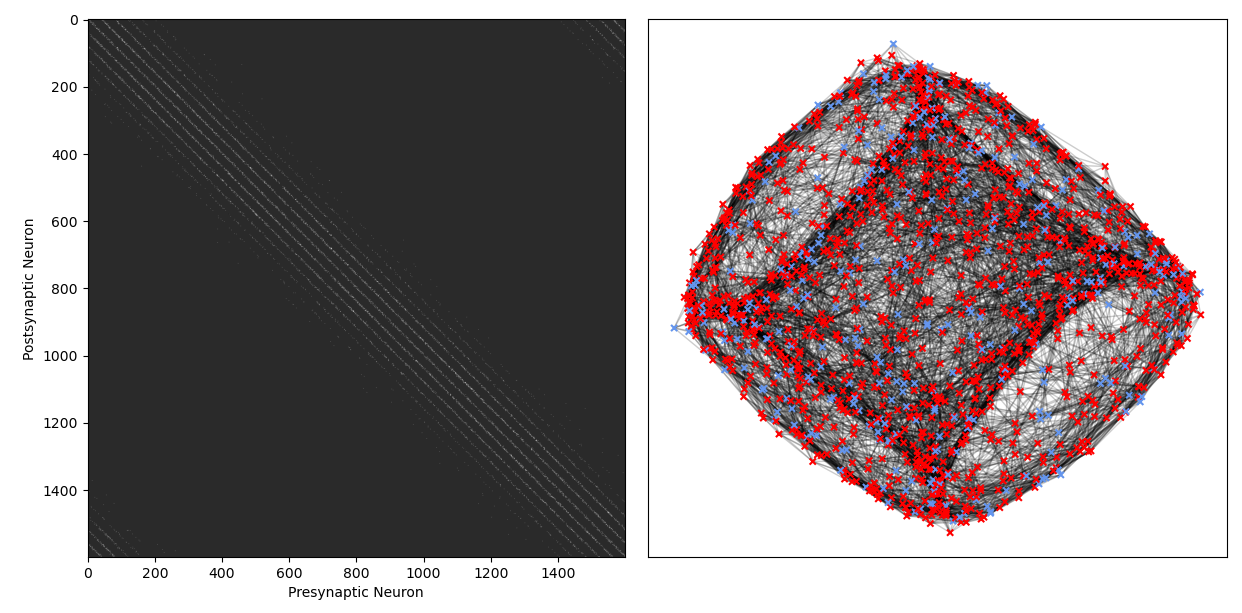
\includegraphics[width=150mm]{fig_5-A}
\caption{An example 2D gaussian lattice model with periodic boundary conditions}
\end{figure}

Significant effort has been spent in recent years to map the connectivity patterns of networks in cortex and thus variety of models have appeared. Connection patterns have been quantified by calculating a broad range of structural measures, including small-world attributes and motif composition, as well as some global measures of functional connectivity (Sporns 2006). The structural measures defined in this framework have proven quite useful; however, many models are defined without consideration of the fact that cortical networks are embedded in real space. In principle these spatially-dependent connectivity patterns could be hidden in the topology of an arbitrary graph; however, in some cases it is more straightforward to interpret connectivity patterns in the spatial domain. For example, the connectivity in a 2D lattice of LIF neurons with local and global synaptic connections are readily understood in terms of distances in real space (Rosenbaum 2014). At the same time, theoretical models e.g., mean-field theories of network dynamics have relaxed the strong assumption that cortical networks are spatially homogeneous (Brunel 2000). Defining a periodic connectivity kernel for each neuron on a lattice is an attractive model for cortical networks as it accurately describes the invariance of connectivity to translations. In other words, each neuron in the network has a similiar input and output structure - a property which drastically simplifies theoretical calculations.


\chapter{Sampling from the posterior}

This family of techniques, often formally referred to as Langevin dynamics, is defined by the use of stochastic differential equations to model the evolution of systems with high degrees of freedom. A Fokker-Planck equation allows us to solve for the time evolution of the probability distribution over such a variable, providing insights into the dynamics which cannot be seen from any one trajectory through the space of states. 


\section{The diffusion approximation on the 2D Gaussian lattice}

The moments $M_{n}(t)$ derived above in the Kramers-Moyal expansion are dependent on the connectivity of the network and the statistics of the input. We will first consider a classic case, where we have a sparse directed network with constant synaptic efficacy between all presynaptic and postsynaptic pairs of cells. This primary pool of neurons is subject to stimulation by $N_{\mathrm{in}}$ input neurons with a connection probability $\gamma_{\mathrm{in}}$ giving $C_{\mathrm{in}} = \gamma_{\mathrm{in}}N_{\mathrm{rec}}$ unique connections between the input population and a single neuron in the recurrent pool. Within the recurrent pool, we have a connection probability of $\gamma_{\mathrm{rec}} << 1$ for any pair giving $C_{\mathrm{rec}} = \gamma_{\mathrm{rec}} N_{\mathrm{rec}}$ recurrent inputs per postsynaptic cell. We assume that a presynaptic action potential invokes a post synaptic potential (PSP) with magnitude $J_{0}$ in the postsynaptic cell with $J_{0} << \theta$ for both input and recurrent projections. The first moment of the transition operator $T(V',t| V,t-\tau)$ is given by

\begin{align*}
\mu(t) &= \mu_{in} + \mu_{rec}(t)\\
&= \left(C_{\mathrm{in}}\nu_{\mathrm{in}}(t) + C_{\mathrm{rec}}\nu_{\mathrm{rec}}(t)\right)\tau\langle J\rangle\\
&= \left(C_{\mathrm{in}}\nu_{\mathrm{in}}(t) + C_{\mathrm{rec}}\nu_{\mathrm{rec}}(t)\right)\tau J_{0}
\end{align*}

where $\nu_{\mathrm{in}}(t)$ is the rate parameter for the input Poisson process. The second moment

\begin{align*}
\sigma^{2}(t) &= \sigma_{\mathrm{rec}}^{2} + \sigma_{\mathrm{ext}}^{2}\\
&= \left(C_{\mathrm{in}}\nu_{\mathrm{in}}(t) + C_{\mathrm{rec}}\nu_{\mathrm{rec}}(t)\right)\tau\langle J^{2}\rangle\\
&= \left(C_{\mathrm{in}}\nu_{\mathrm{in}}(t) + C_{\mathrm{rec}}\nu_{\mathrm{rec}}(t)\right)\tau J_{0}^{2}
\end{align*}

After inserting the first two moments into (2.10) we arrive at the following Fokker-Planck equation

\begin{align*}
\dot{P}(V,t) &= -\frac{\partial}{\partial V}[\mu(t)P(V,t)] + \frac{1}{2}\frac{\partial^{2}}{\partial V^{2}}[\sigma^{2}(t)P(V,t)]\\
\end{align*} 

At this point, it is necessary to impose the appropriate boundary conditions on the above Fokker-Planck equation as in so as to maintain biological realism. The Fokker-Planck equation can be written as the continuity equation 

\begin{equation*}
\frac{\partial P(v,t)}{\partial t} = -\frac{\partial S}{\partial V}
\end{equation*}

(Risken, 1984) with 

\begin{equation*}
S(V,t) = -\frac{v-V_{L}-\mu}{\tau}P(V,t) - \frac{\sigma^{2}(t)}{2\tau}\frac{\partial P(V,t)}{\partial V}
\end{equation*}

which is known as the \emph{probability current} through voltage $V$ at a time $t$. The instantaneous firing rate is equivalent to the probability current through the threshold i.e. $\nu(t) = S(\theta,t)$. Furthermore, we require that the probability current through the firing threshold $P(\theta, t)=0$ and that instead this probability emerges at the resting potential after a refactory period of $\tau_{\mathrm{ref}}$. This condition gives the following boundary condition for the derivative of the probability with respect to voltage

\begin{equation*}
\frac{\partial P(\theta,t)}{\partial V} = -\frac{2\tau\nu(t)}{\sigma^{2}(t)}
\end{equation*}

To account for the refractory period $\tau_{\mathrm{ref}}$, we define an auxililary distribution

\begin{equation*}
p_{r}(t) = \int_{t-\tau_{\mathrm{ref}}}^{t} \nu(t)dt
\end{equation*}

which together with the distribution $P(V,t)$ satisfy the normalization condition:

\begin{equation*}
\int P(v,t)dV + p_{r}(t) = 1
\end{equation*}

\begin{align*}
\frac{\partial P(v,t)}{\partial t} &= \left(\mu(t) - \frac{v-v_{L}}{\tau}\right) \frac{\partial}{\partial v} P(v,t) - \frac{\sigma^{2}(t)}{2\tau}\frac{\partial^{2}}{\partial v^{2}} P(v,t) + \nu(t-\tau_{\mathrm{ref}})\delta(v-V_{R})\\
\end{align*} 


which we approximate by central finite differences

\begin{align*}
\frac{p(v, t+\Delta t) - p(v,t)}{\Delta t} &= \left(\mu(t) - \frac{v-v_{L}}{\tau}+ \mu_{ext}\right)\frac{p(v+\Delta v, t) - p(v,t)}{\Delta v} \\
&- \frac{1}{2}\left(\sigma^{2}(t) + \sigma_{ext}^{2}\right)\frac{p(v+\Delta v, t) - 2p(v,t) + p(v-\Delta v, t)}{\Delta v^{2}}
\end{align*} 

We consider a general network of $N$ leaky integrate and fire units expressed mathematically as a weighted graph $\mathcal{N}$. We defined the state vector $\mathbf{V}$ that stores the membrane potential of each cell, which evolves according to a set of $N$ coupled differential equations

\begin{align*}
\dot{V_{j}}(t) = -\frac{V_{j}(t)}{\tau} + \sum_{i}J_{ij}\delta(t-t_{spike}) + X_{j}(t)
\end{align*}

for a stochastic input $X$, which we assume can be written as a compound Poisson process, and a weighted summation of spikes in the primary population $\sum_{i}J_{ij}\delta(t-t_{spike})$. The state vector for the system is then $\mathbf{V}(t) = (V_{0}(t), V_{1}(t), ..., V_{N}(t))$ and we look for an analytical relationship between the joint distribution $P(\mathbf{V}(t))$ and the synaptic connectivity $J$. In principle, if we know the moments $\{M_{j}^{n}\}$  of the transition operator $T_{j}(V',t'|V,t)$ for every neuron $j$ to arbitrary order, we can express $\dot{P}(\mathbf{V}(t))$ according to the KM expansion in (2.7). The primary hurdle we need to overcome in this procedure then becomes relating the moments $\{M_{j}^{n}\}$ to the synaptic connectivity $J$. For example, we can construct a general template for the distribution $T_{j}$ by noticing that the probability of a binary input pattern

\begin{align*}
P(\mathbf{z}) = \underset{j}{\prod} \; p_{j}^{z_{j}}(1-p_{j})^{1-z_{j}}
\end{align*}

which is a multivariate Bernoulli distribution. If we let $\xi$ index the space of possible binary patterns

\begin{align}
T(V',t'|V,t) = \sum_{\xi} \delta(V'- V - J\cdot z_{\xi})\underset{j}{\prod} \; p_{j}^{z_{j}}(1-p_{j})^{1-z_{j}}
\end{align}

so we see that we must first know $P(\mathbf{z})$ which in turn requires knowledge of all $p_{j} = P_{j}(\theta, t)$ i.e. the probability flux at the threshold $\theta$. We now argue that the moments of (2.8) can be found 

\begin{align}
M_{n} = \int (V-V')^{n} T(V',t'|V,t) dV
\end{align}

which are essentially the moments of a compound Bernoulli distribution where the individual probabilities $p_{j}(t')$ are given by $P_{j}(\theta, t)$.


\begin{appendices}
\chapter{The Kramers-Moyal expansion}

Given many instantiations of a stochastic variable $V$, we can construct a normalize histogram over all observations as a function of time $P(V,t)$. However, in order to systematically explore the relationship between the parameterization of the process and $P(V,t)$ we require an expression for $\dot{P}(V,t)$. If we make a fundamental assumption that the evolution of $P(V,t)$ follows a Markov process i.e. its evolution has the memoryless property, then we can write

\begin{equation}
P(V', t) = \int T(V', t | V, t-\tau)P(V, t-\tau)dV
\end{equation} 

which is known at the Chapman-Kolmogorov equation. The factor $T(V', t | V, t-\tau)$ is known as the \emph{transition operator} in a Markov process and determines the evolution of $P(V,t)$ in time. We proceed by writing $T(V', t | V, t-\tau)$ in a form referred to as the Kramers-Moyal expansion

\begin{align*}
T(V', t | V, t-\tau) &= \int \delta(u-V')T(u, t | V, t-\tau)du\\
&= \int \delta(V+u-V'-V)T(u, t | V, t-\tau)du\\
\end{align*} 

If we use the Taylor expansion of the $\delta$-function 

\begin{equation*}
\delta(V+u-V'-V) = \sum_{n=0}^{\infty} \frac{(u-V)^{n}}{n!}\left(-\frac{\partial}{\partial V}\right)^{n}\delta(V-V')
\end{equation*}

Inserting this into the result from above, pulling out terms independent of $u$ and swapping the order of the sum and integration gives

\begin{align}
T(V', t | V, t-\tau) &= \sum_{n=0}^{\infty} \frac{1}{n!}\left(-\frac{\partial}{\partial V}\right)^{n}\delta(V-V')\int(u-V)^{n}T(u, t | V, t-\tau)du\\
&= \sum_{n=0}^{\infty} \frac{1}{n!}\left(-\frac{\partial}{\partial V}\right)^{n}\delta(V-V')M_{n}(V,t)
\end{align} 

noticing that $M_{n}(V,t) = \int(u-V)^{n}T(u, t | V, t-\tau)du$ is just the $n$th moment of the transition operator $T$. Plugging (2.6) back in to (2.4) gives 

\begin{align}
P(V, t) &= \int \left(1 + \sum_{n=1}^{\infty} \frac{1}{n!}\left(-\frac{\partial}{\partial V}\right)^{n} M_{n}(V,t)\right)\delta(V-V')P(V, t-\tau)dV\\
&= P(V', t-\tau) + \sum_{n=1}^{\infty} \frac{1}{n!}\left(-\frac{\partial}{\partial V}\right)^{n} \left[M_{n}(V,t)P(V,t)\right]
\end{align} 

Approximating the derivative as a finite difference and taking the limit $\tau\rightarrow 0$ gives

\begin{align}
\dot{P}(V,t)  &= \underset{\tau\rightarrow 0}{\mathrm{lim}}\left(\frac{P(V, t)-P(V, t-\tau)}{\tau}\right)\\
&= \sum_{n=1}^{\infty} \frac{1}{n!}\left(-\frac{\partial}{\partial V}\right)^{n} \left[M_{n}(V,t)P(V,t)\right]
\end{align} 

which is formally known as the Kramers-Moyal (KM) expansion. The Fokker-Planck equation is a special case of (2.10) where we neglect terms $n>2$ in the \emph{diffusion approximation}.
\end{appendices}

% Format a LaTeX bibliography
\makebibliography

[1] D.O. Hebb \textit{The organization of behavior: A neurophysiological theory}. John Wiley and Sons. 1949.

% Figures and tables, if you decide to leave them to the end
%\input{figure}
%\input{table}

\end{document}


